\chapter{Dimensionality Reduction and Representation}
\label{ch:dimred}

\chapterguide%
  {\chapref{ch:unsupervised}, dot products and projections from \chapref{ch:foundations}, and scaling from \chapref{ch:data}. Eigenvectors and eigenvalues are re-introduced from scratch here.}
  {compute PCA, choose components, assess information loss, and interpret nonlinear visualizations cautiously.}

Dimensionality reduction compresses redundant features while preserving a stated property, such as variance or neighborhoods. It can support visualization, denoising, faster models, and more manageable geometry (\chapref{ch:knn-nb}).

\section{The idea: find better axes}

A cloud of correlated points does not use its dimensions efficiently --- most of the action happens along a few directions. Principal component analysis (PCA) rotates the coordinate system to point along those directions.

\begin{mlfigure}
\begin{tikzpicture}
\begin{axis}[
  width=0.80\linewidth, height=6.2cm,
  axis lines=middle,
  xlabel={$x_1$}, ylabel={$x_2$},
  ticks=none, xmin=-2.9, xmax=2.9, ymin=-2.7, ymax=2.7,
  clip=false
]
\addplot[only marks, mark=*, mark size=1.6pt] coordinates {
  (-2,-1.6) (-1.4,-1.1) (-0.6,-0.2) (0,0.3) (0.7,0.4)
  (1.3,1.2) (2,1.7) (-0.2,-0.5) (1.7,1.9) (-1.8,-2.0)
};
\draw[-{Stealth[length=2.4mm]}, very thick]
  (axis cs:0,0) -- (axis cs:2.0,1.6)
  node[right, font=\small] {PC1: most variance};
\draw[-{Stealth[length=2.4mm]}, thick]
  (axis cs:0,0) -- (axis cs:-0.64,0.8)
  node[above, font=\small] {PC2};
\end{axis}
\end{tikzpicture}
\end{mlfigure}

\begin{intuition}
Think of photographing a school of fish. From most angles the school looks like a blob, but from one particular angle its long axis lines up with the frame and one photo captures almost everything. PCA finds that best camera angle: the first principal component is the direction along which the data is most spread out, the second is the most-spread direction perpendicular to the first, and so on.
\end{intuition}

% === VISUAL ADDITION: pca-rotate-project ===
\subsection{PCA as rotate, then project}

The first component is not merely an arrow drawn on the old graph. It becomes a new coordinate axis, and every observation receives a new number: its position along that axis.

\begin{mlfigure}
\begin{tikzpicture}[font=\scriptsize,scale=0.86]
\def\cloud{
  (-1.7,-1.35),(-1.25,-0.85),(-0.8,-0.72),(-0.25,-0.05),
  (0.25,0.18),(0.7,0.48),(1.15,1.02),(1.65,1.28)
}
% original
\begin{scope}
  \draw[-{Stealth[length=1.8mm]},MLMuted] (-2.0,0) -- (2.05,0) node[right] {$x_1$};
  \draw[-{Stealth[length=1.8mm]},MLMuted] (0,-1.75) -- (0,1.75) node[above] {$x_2$};
  \foreach \p in \cloud \fill[MLBlue] \p circle (2.2pt);
  \node[font=\small\bfseries\color{MLNavy}] at (0,2.15) {1. Original coordinates};
\end{scope}

% rotated direction
\begin{scope}[xshift=5.15cm]
  \draw[MLMuted!45] (-2.0,0) -- (2.0,0);
  \draw[MLMuted!45] (0,-1.75) -- (0,1.75);
  \foreach \p in \cloud \fill[MLBlue] \p circle (2.2pt);
  \draw[-{Stealth[length=2mm]},MLTeal,very thick] (-1.75,-1.35) -- (1.82,1.40)
    node[right,font=\scriptsize] {PC1};
  \draw[-{Stealth[length=2mm]},MLOrange,thick] (0.75,-0.98) -- (-0.75,0.98)
    node[above,font=\scriptsize] {PC2};
  \node[font=\small\bfseries\color{MLNavy}] at (0,2.15) {2. Rotate to principal axes};
\end{scope}

% projected 1d
\begin{scope}[xshift=10.25cm]
  \draw[-{Stealth[length=1.8mm]},MLTeal,very thick] (-2.0,0) -- (2.05,0) node[right] {PC1 score};
  \foreach \x in {-1.72,-1.22,-0.86,-0.22,0.28,0.72,1.20,1.68}
    \fill[MLBlue] (\x,0) circle (2.3pt);
  \draw[MLMuted,dashed] (-2.0,0.65) -- (2.0,0.65);
  \node[align=center,text=MLMuted] at (0,1.03) {PC2 discarded};
  \node[font=\small\bfseries\color{MLNavy}] at (0,2.15) {3. Project to one dimension};
  \node[align=center,text=MLGreen] at (0,-0.72) {two columns become\\one component score};
\end{scope}
\end{tikzpicture}
\end{mlfigure}
% === END VISUAL ADDITION ===

\section{PCA step by step}

\begin{enumerate}
  \item \term{Center} the data by subtracting each feature's training mean. Decide separately whether to standardize: do so when equal standardized variation should carry equal weight, but retain original units when their variance is scientifically meaningful.
  \item Compute the sample covariance matrix
  \[
    S=\frac{1}{n-1}X^{\mathsf T}X
  \]
  for the centered matrix $X$.
  \item Find its eigenvectors and eigenvalues: for centered data matrix $X$,
  \[
    S\bm{v}=\lambda\,\bm{v}.
  \]
  Each eigenvector $\bm{v}$ is a component direction; its eigenvalue $\lambda$ measures the variance captured along it.
  \item \term{Sort} components by eigenvalue and keep the top $k$.
  \item \term{Project}: the new features (\term{scores}) are the dot products of each observation with the kept components.
\end{enumerate}

The proportion of variance explained by component $j$ is
\[
  \frac{\lambda_j}{\sum_{k}\lambda_k},
\]
explaining the variance along each axis, not its predictive value (\secref{sec:pca-limitations}). Components are orthogonal and fitted scores uncorrelated. SVD of centered data computes the same directions.

\begin{workedexample}
Take five centered points that lie exactly on a line: $(-2,-2)$, $(-1,-1)$, $(0,0)$, $(1,1)$, $(2,2)$. Each feature has variance $10/4=2.5$ and their covariance is also $2.5$, so the covariance matrix is
$\begin{bsmallmatrix}2.5 & 2.5\\ 2.5 & 2.5\end{bsmallmatrix}$
with $\lambda_1=5$, $\lambda_2=0$, and $\bm v_1=(1,1)/\sqrt2$. Scores $(-2.83,-1.41,0,1.41,2.83)$ retain 100\% of variance in one dimension. Dropping nonzero components instead loses variance.
\end{workedexample}

\section{Explained variance: the compression budget}

\begin{mlfigure}
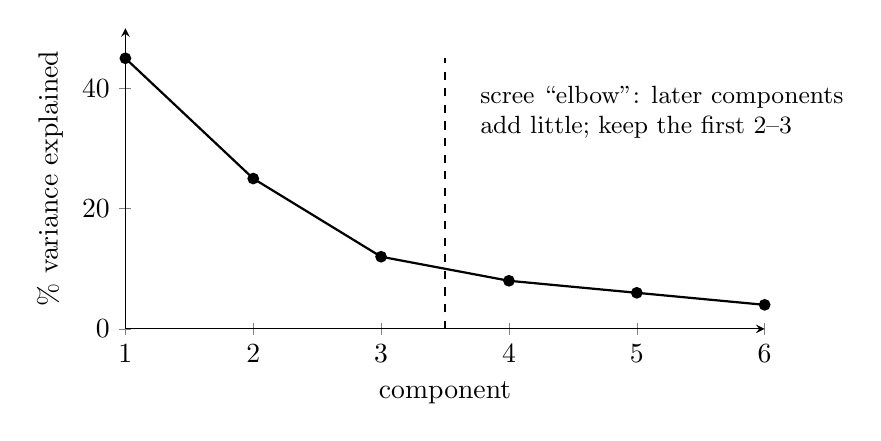
\begin{tikzpicture}
\begin{axis}[
  width=0.80\linewidth, height=5.4cm,
  axis lines=left,
  xlabel={component}, ylabel={\% variance explained},
  xtick={1,2,3,4,5,6},
  ymin=0, ymax=50, clip=false
]
\addplot[thick, mark=*, mark size=1.7pt] coordinates
  {(1,45) (2,25) (3,12) (4,8) (5,6) (6,4)};
\draw[dashed] (axis cs:3.5,0) -- (axis cs:3.5,45);
\node[font=\small, align=left, anchor=west] at (axis cs:3.7,36)
  {scree ``elbow'': later components\\add little; keep the first 2--3};
\end{axis}
\end{tikzpicture}
\end{mlfigure}

Choose components by a variance target, scree plot, or downstream training-fold validation. In Lab~4, 29 of 64 digit components retain 95\% of variance without reducing test accuracy. Discarded eigenvalues sum to lost variance.

\subsection{What PCA cannot promise}
\label{sec:pca-limitations}

\begin{itemize}
  \item It is \term{linear}: a spiral or a curved sheet of data has structure PCA cannot straighten out.
  \item It is \term{scale-sensitive}: changing units changes the covariance matrix. Standardize when that influence is arbitrary, not as an automatic rule.
  \item \term{Variance is not predictive importance}: low-variance directions may carry label signal. LDA instead seeks class separation (\chapref{ch:classification}).
  \item \term{Interpretation}: inspect component weights; each component blends original features.
\end{itemize}

\begin{pitfall}
Projecting a four-feature clustering into two PCA dimensions only visualizes its existing assignments. Clustering the two PCA columns instead is a different model with reduced information.
\end{pitfall}

\section{Choosing the component count in practice}

\begin{mlfigure}
\begin{tikzpicture}[baseline=(current bounding box.north)]
\begin{axis}[
  width=0.46\linewidth, height=4.3cm, axis lines=left,
  title style={font=\small\bfseries\color{MLNavy}}, title={Variance per component},
  xlabel={Component}, ylabel={Share of variance},
  label style={font=\scriptsize\color{MLMuted}}, tick label style={font=\scriptsize\color{MLMuted}},
  ybar, bar width=7pt, ymin=0, ymax=0.5, xmin=0.3, xmax=10.7
]
\addplot[fill=MLPaleBlue,draw=MLBlue] coordinates
  {(1,0.42)(2,0.23)(3,0.13)(4,0.08)(5,0.05)(6,0.035)(7,0.02)(8,0.015)(9,0.008)(10,0.002)};
\end{axis}
\end{tikzpicture}
\hfill
\begin{tikzpicture}[baseline=(current bounding box.north)]
\begin{axis}[
  width=0.46\linewidth, height=4.3cm, axis lines=left,
  title style={font=\small\bfseries\color{MLNavy}}, title={Cumulative variance kept},
  xlabel={Number of components}, ylabel={Total kept},
  label style={font=\scriptsize\color{MLMuted}}, tick label style={font=\scriptsize\color{MLMuted}},
  ymin=0, ymax=1.05, xmin=0.5, xmax=10.5
]
\addplot[MLTeal,very thick,mark=*,mark size=1.4pt] coordinates
  {(1,0.42)(2,0.65)(3,0.78)(4,0.86)(5,0.91)(6,0.945)(7,0.965)(8,0.98)(9,0.988)(10,0.99)};
\draw[MLRed,thick,dashed] (axis cs:0.5,0.9) -- (axis cs:10.5,0.9);
\draw[MLRed,thick,dashed] (axis cs:5,0) -- (axis cs:5,0.9);
\node[font=\scriptsize\color{MLRed},anchor=west] at (axis cs:5.3,0.55) {5 components hold 91\%};
\end{axis}
\end{tikzpicture}
\end{mlfigure}

\begin{analogy}
PCA chooses viewing directions with the greatest variance, each orthogonal to the previous ones. A scree plot shows how much each additional direction contributes.
\end{analogy}

\section{t-SNE and UMAP: maps for the eye}
\label{sec:tsne-umap}

For two-dimensional neighborhood maps rather than global variance preservation, consider t-SNE or UMAP.

\term{t-SNE} converts distances into neighbor probabilities and arranges points in 2-D so that neighborhoods are preserved: points close in the original space stay close on the map. Its main hyperparameter, \term{perplexity}, roughly sets the neighborhood size being honored (typical values 5--50).

\term{UMAP} pursues the same goal with different mathematics; it is much faster, tends to preserve somewhat more of the global arrangement, and --- unlike classic t-SNE --- can place \emph{new} points onto an existing map.

Both need cautious reading:

\begin{itemize}
  \item cluster sizes, empty gaps, and distances between separated groups can be artifacts; even apparent neighborhoods should be checked against original-space distances;
  \item check whether the interpretation survives changes in seeds and hyperparameters;
  \item apparent clusters need independent stability and domain evidence;
  \item for ordinary predictive preprocessing, PCA is the simpler default because it has an explicit out-of-sample projection. Nonlinear embeddings need a justified validation design.
\end{itemize}

\begin{mltable}
\begin{tabular}{@{}p{0.3\linewidth}p{0.27\linewidth}p{0.31\linewidth}@{}}
\toprule
\rowcolor{MLPaleBlue!92}
 & PCA & t-SNE / UMAP \\
\midrule
Preserves & global variance, linear structure & local neighborhoods \\
Deterministic? & yes & no (seed-dependent) \\
Handles new points & yes (a projection) & UMAP yes; t-SNE awkwardly \\
Best use & preprocessing, compression, denoising & exploratory visualization \\
\bottomrule
\end{tabular}
\end{mltable}

PCA, t-SNE, and UMAP \term{extract} new features; \term{selection} retains original columns (\secref{sec:feature-selection}).

\begin{keyidea}
PCA quantifies lost variance; nonlinear maps emphasize neighborhoods and need cautious interpretation. A visualization is evidence to investigate, not a substitute for the original data.
\end{keyidea}

\begin{modelcard}{Dimensionality Reduction - Quick Guide}
\begin{tabularx}{\linewidth}{@{}>{\bfseries\leavevmode\color{MLNavy}}p{0.24\linewidth}X@{}}
PCA is best for & Compressing correlated numerical features, denoising, visualization, and faster downstream modeling. \cr
Preprocessing & Center features; standardize when unit scales are arbitrary and equal standardized influence is intended. \cr
Main control & Number of components, chosen by explained variance and downstream validation. \cr
Visualization tools & t-SNE and UMAP can create useful two-dimensional maps of local neighborhoods. \cr
Watch for & Loss of interpretability, information loss, leakage from fitting on all data, and over-interpreting visual clusters. \cr
\end{tabularx}
\end{modelcard}

\labsection{4}{Unsupervised learning I: clustering and PCA}{sec:lab04-clustering-pca}

\begin{labproject}{Find structure without an answer key}
\textbf{Goal.} Choose $K$ from evidence, compare DBSCAN, and evaluate PCA through reconstruction and downstream accuracy.

\medskip\noindent\textbf{Setup.}\par
\begin{lstlisting}[style=mlpython]
import zipfile
from pathlib import Path

import joblib
import matplotlib.pyplot as plt
import numpy as np
import pandas as pd
from sklearn.cluster import DBSCAN, KMeans
from sklearn.decomposition import PCA
from sklearn.linear_model import LogisticRegression
from sklearn.metrics import accuracy_score, silhouette_score
from sklearn.model_selection import train_test_split
from sklearn.pipeline import Pipeline
from sklearn.preprocessing import StandardScaler

PROJECT_ROOT = Path.cwd().parent
DATA = PROJECT_ROOT / "all_datasets"
MODELS = PROJECT_ROOT / "models"
MODELS.mkdir(exist_ok=True)
\end{lstlisting}

\medskip\noindent\textbf{Part A --- How many clusters? Elbow and silhouette.}\par

Standardize age, income, and spending score for 200 mall customers; investigate useful segments without labels.

\begin{lstlisting}[style=mlpython]
customers = pd.read_csv(DATA / "mall_customers_dataset.csv")
print(customers.head())

features = ["Age", "Annual Income (k$)", "Spending Score (1-100)"]
X = StandardScaler().fit_transform(customers[features])
\end{lstlisting}

Try $K=2$--8. Inertia measures within-cluster squared distances and falls with $K$; silhouette measures cohesion versus separation.

\begin{lstlisting}[style=mlpython]
ks, inertias, silhouettes = [], [], []
for k in range(2, 9):
    kmeans = KMeans(n_clusters=k, n_init=20, random_state=42)
    labels = kmeans.fit_predict(X)
    ks.append(k)
    inertias.append(kmeans.inertia_)
    silhouettes.append(silhouette_score(X, labels))
    print(f"k={k}  inertia={kmeans.inertia_:.1f}  silhouette={silhouettes[-1]:.3f}")

fig, axes = plt.subplots(1, 2, figsize=(9.5, 3.4))
axes[0].plot(ks, inertias, marker="o")
axes[0].set_xlabel("Number of clusters k")
axes[0].set_ylabel("Inertia")
axes[0].set_title("Elbow: look for the bend")
axes[1].plot(ks, silhouettes, marker="o")
axes[1].set_xlabel("Number of clusters k")
axes[1].set_ylabel("Silhouette score")
axes[1].set_title("Silhouette: look for the peak")
plt.tight_layout()
plt.show()
\end{lstlisting}

\textbf{Inspect.} Inertia and silhouette suggest five or six groups; domain usefulness must guide the choice.

\medskip\noindent\textbf{Part B --- K-means versus DBSCAN.}\par

$K$-means assigns every customer. DBSCAN uses radius and neighbor count, leaving noise labeled $-1$.

\begin{lstlisting}[style=mlpython]
kmeans = KMeans(n_clusters=5, n_init=30, random_state=42)
k_labels = kmeans.fit_predict(X)
print("K-means silhouette:", round(silhouette_score(X, k_labels), 3))

dbscan = DBSCAN(eps=0.75, min_samples=6)
d_labels = dbscan.fit_predict(X)
is_clustered = d_labels != -1
n_clusters = len(set(d_labels[is_clustered]))
print("DBSCAN clusters:", n_clusters, " noise points:", int((~is_clustered).sum()))
if n_clusters >= 2:
    print("DBSCAN silhouette (clustered points only):",
          round(silhouette_score(X[is_clustered], d_labels[is_clustered]), 3))
\end{lstlisting}

Describe clusters using means of the original features.

\begin{lstlisting}[style=mlpython]
segments = customers.copy()
segments["kmeans_cluster"] = k_labels
segments["dbscan_cluster"] = d_labels
profile = segments.groupby("kmeans_cluster")[features].mean().round(1)
profile["customers"] = segments["kmeans_cluster"].value_counts().sort_index()
print(profile)
\end{lstlisting}

\begin{lstlisting}[style=mlpython]
fig, axes = plt.subplots(1, 2, figsize=(10, 3.9))
panels = [(axes[0], k_labels, "K-means, k = 5"),
          (axes[1], d_labels, "DBSCAN, eps = 0.75 (noise = -1)")]
for ax, labels, title in panels:
    scatter = ax.scatter(customers["Annual Income (k$)"], customers["Spending Score (1-100)"],
                         c=labels, cmap="tab10", alpha=0.8)
    ax.set_xlabel("Annual income (k$)")
    ax.set_ylabel("Spending score")
    ax.set_title(title)
    ax.legend(*scatter.legend_elements(), title="cluster", fontsize=8, loc="center right")
plt.tight_layout()
plt.show()
\end{lstlisting}

\textbf{Inspect.} $K$-means partitions income/spending segments; DBSCAN at this radius finds one cloud plus noise. Different grouping assumptions explain the contrast. Try a smaller \texttt{eps}.

\medskip\noindent\textbf{Part C --- PCA as compression, judged by a downstream model.}\par

Each digit has $8\times8=64$ pixels. Use the official training split; reserve test evaluation until the final comparison.

\begin{lstlisting}[style=mlpython]
archive_path = DATA / "optical_recognition_handwritten_digits.zip"
columns = [f"pixel_{i}" for i in range(64)] + ["label"]
with zipfile.ZipFile(archive_path) as archive:
    members = {Path(name).name: name for name in archive.namelist()}
    train = pd.read_csv(archive.open(members["optdigits.tra"]), header=None, names=columns)
    test = pd.read_csv(archive.open(members["optdigits.tes"]), header=None, names=columns)

X_dev = train.drop(columns="label") / 16.0     # pixel values 0-16 -> 0-1
y_dev = train["label"]
X_test = test.drop(columns="label") / 16.0
y_test = test["label"]
print("training digits:", len(X_dev), " test digits:", len(X_test))

fig, axes = plt.subplots(1, 10, figsize=(10, 1.4))
for ax, (_, row), label in zip(axes, X_dev.head(10).iterrows(), y_dev.head(10)):
    ax.imshow(row.to_numpy().reshape(8, 8), cmap="gray_r")
    ax.set_title(str(label), fontsize=9)
    ax.axis("off")
plt.suptitle("The first ten training digits (8 x 8 pixels each)", y=1.05)
plt.show()
\end{lstlisting}

Validate PCA budgets retaining 90\%, 95\%, or 99\% variance through classifier accuracy on training-file holdouts.

\begin{lstlisting}[style=mlpython]
X_fit, X_valid, y_fit, y_valid = train_test_split(
    X_dev, y_dev, test_size=0.25, random_state=42, stratify=y_dev
)

baseline = LogisticRegression(max_iter=2000).fit(X_fit, y_fit)
print("all 64 pixels: validation accuracy =",
      round(accuracy_score(y_valid, baseline.predict(X_valid)), 4))

for retained_variance in [0.90, 0.95, 0.99]:
    candidate = Pipeline([
        ("pca", PCA(n_components=retained_variance, svd_solver="full")),
        ("model", LogisticRegression(max_iter=2000)),
    ])
    candidate.fit(X_fit, y_fit)
    n_kept = candidate.named_steps["pca"].n_components_
    print(f"{retained_variance:.0%} variance: {n_kept:2d} components, "
          f"validation accuracy = {accuracy_score(y_valid, candidate.predict(X_valid)):.4f}")
\end{lstlisting}

Lock 95\%, refit both PCA and full-pixel pipelines on all training rows, then compare once on the official test file.

\begin{lstlisting}[style=mlpython]
final_model = Pipeline([
    ("pca", PCA(n_components=0.95, svd_solver="full")),
    ("model", LogisticRegression(max_iter=2000)),
])
final_model.fit(X_dev, y_dev)
full_model = LogisticRegression(max_iter=2000).fit(X_dev, y_dev)
pca = final_model.named_steps["pca"]

print("\nFINAL TEST (official test file)")
print("all 64 pixels accuracy:", round(accuracy_score(y_test, full_model.predict(X_test)), 4))
print("PCA components kept:", pca.n_components_,
      " variance retained:", round(pca.explained_variance_ratio_.sum(), 4))
print("PCA -> logistic accuracy:", round(accuracy_score(y_test, final_model.predict(X_test)), 4))
\end{lstlisting}

Reconstruct test digits from component scores and inspect cumulative explained variance.

\begin{lstlisting}[style=mlpython]
reconstructed = pca.inverse_transform(pca.transform(X_test.head(8)))

fig, axes = plt.subplots(2, 8, figsize=(9, 2.6))
for j in range(8):
    axes[0, j].imshow(X_test.iloc[j].to_numpy().reshape(8, 8), cmap="gray_r")
    axes[1, j].imshow(reconstructed[j].reshape(8, 8), cmap="gray_r")
    axes[0, j].axis("off")
    axes[1, j].axis("off")
axes[0, 0].set_title("original (64 numbers)", fontsize=8, loc="left")
axes[1, 0].set_title(f"rebuilt from {pca.n_components_} components", fontsize=8, loc="left")
plt.show()

plt.figure(figsize=(5.5, 3.4))
all_components = PCA(svd_solver="full").fit(X_dev)
plt.plot(np.arange(1, 65), np.cumsum(all_components.explained_variance_ratio_), marker=".")
plt.axhline(0.95, linestyle="--", color="grey")
plt.axvline(pca.n_components_, linestyle="--", color="grey")
plt.xlabel("Number of principal components")
plt.ylabel("Cumulative explained variance")
plt.title("Most of the picture lives in the first 30 directions")
plt.tight_layout()
plt.show()
\end{lstlisting}

\textbf{Inspect.} Reconstructions blur slightly while accuracy holds. The last 35 components carry under 5\% of variance.

Save PCA and classifier together to accept new 64-pixel images.

\begin{lstlisting}[style=mlpython]
model_path = MODELS / "digits_pca_logistic.joblib"
joblib.dump(final_model, model_path)

loaded = joblib.load(model_path)
first_digits = X_test.iloc[:5]
print("predicted:", loaded.predict(first_digits).tolist())
print("actual:   ", y_test.iloc[:5].tolist())
\end{lstlisting}

\begin{tryit}
Set DBSCAN \texttt{eps=0.5}; count clusters/noise and justify which result better serves marketing.
\end{tryit}
\end{labproject}


\begin{quickcheck}
\begin{enumerate}
  \item What does PCA optimize when it chooses its first principal component?
  \item Why can standardization change which PCA directions appear most important?
  \item Why should distances and apparent cluster sizes in a t-SNE or UMAP plot not be interpreted as exact properties of the original high-dimensional data?
\end{enumerate}
\end{quickcheck}
